% mnras_template.tex
%
% LaTeX template for creating an MNRAS paper
%
% v3.0 released 14 May 2015
% (version numbers match those of mnras.cls)
%
% Copyright (C) Royal Astronomical Society 2015
% Authors:
% Keith T. Smith (Royal Astronomical Society)

% Change log
%
% v3.0 May 2015
%    Renamed to match the new package name
%    Version number matches mnras.cls
%    A few minor tweaks to wording
% v1.0 September 2013
%    Beta testing only - never publicly released
%    First version: a simple (ish) template for creating an MNRAS paper

%%%%%%%%%%%%%%%%%%%%%%%%%%%%%%%%%%%%%%%%%%%%%%%%%%
% Basic setup. Most papers should leave these options alone.
\documentclass[a4paper,fleqn,usenatbib]{mnras}

% MNRAS is set in Times font. If you don't have this installed (most LaTeX
% installations will be fine) or prefer the old Computer Modern fonts, comment
% out the following line
%\usepackage{newtxtext,newtxmath}
% Depending on your LaTeX fonts installation, you might get better results with one of these:
%\usepackage{mathptmx}
%\usepackage{txfonts}

% Use vector fonts, so it zooms properly in on-screen viewing software
% Don't change these lines unless you know what you are doing
\usepackage[T1]{fontenc}
\usepackage{ae,aecompl}



%%%%% AUTHORS - PLACE YOUR OWN PACKAGES HERE %%%%%

% Only include extra packages if you really need them. Common packages are:
\usepackage{graphicx}	% Including figure files
\usepackage{amsmath}	% Advanced maths commands
\usepackage{amssymb}	% Extra maths symbols

%%%%%%%%%%%%%%%%%%%%%%%%%%%%%%%%%%%%%%%%%%%%%%%%%%

%%%%% AUTHORS - PLACE YOUR OWN COMMANDS HERE %%%%%

% Please keep new commands to a minimum, and use \newcommand not \def to avoid
% overwriting existing commands. Example:
%\newcommand{\pcm}{\,cm$^{-2}$}	% per cm-squared

%%%%%%%%%%%%%%%%%%%%%%%%%%%%%%%%%%%%%%%%%%%%%%%%%%

%%%%%%%%%%%%%%%%%%% TITLE PAGE %%%%%%%%%%%%%%%%%%%

% Title of the paper, and the short title which is used in the headers.
% Keep the title short and informative.
\title[]{Efficiently sampling rare events in population synthesis models}

% The list of authors, and the short list which is used in the headers.
% If you need two or more lines of authors, add an extra line using \newauthor
\author[]{Floor Broekgaarden et al. ,$^{1,2}$\thanks{E-mail: fsbroekgaarden@gmail.com}
(TBD)
%Stephen Justham,$^{1,2}$
%Ilya Mandel$^{1,3}$
%Jonathan Gair$^{1,4}$ \newauthor
%Tassos Fragos$^{1,5}$
\\
% List of institutions
$^{1}$Dark Cosmology Centre, Niels Bohr Institute, University of
Copenhagen, Juliane Maries Vej 30, DK-2100, K\o benhaven \o,
Denmark\\
$^{2}$ Astronomical Institute Anton Pannekoek, University of Amsterdam, P.O. Box 94249, 1090 GE, Amsterdam, The Netherlands \\
%$^{2}$Kavli Institute for Astronomy and Astrophysics, Peking University,
%Beijing, China\\
%$^{3}$School of Physics and Astronomy, University of Birmingham, Birmingham B15 2TT, UK\\
%$^{4}$School of Mathematics, University of Edinburgh, The King`s Buildings, Peter
%Guthrie Tait Road, Edinburgh, EH9 3FD, UK
% \\
%$^{5}$Geneva Observatory, University of Geneva, Chemin des Maillettes 51,
%1290 Sauverny, Switzerland
}

% These dates will be filled out by the publisher
%\date{Accepted XXX. Received YYY; in original form ZZZ}

% Enter the current year, for the copyright statements etc.
\pubyear{2017}

% Don't change these lines
\begin{document}
\label{firstpage}
\pagerange{\pageref{firstpage}--\pageref{lastpage}}
\maketitle

% Abstract of the paper
\begin{abstract}
We present an adaptive importance sampling method that can significantly enhance stellar evolution simulations, especially when considering rare events. Simulations often involve calculating integrals over the initial parameter space, e.g. when calculating the fraction of binary black hole mergers. The method presented here estimates the wanted outcome by drawing samples from an instrumental distribution that is adaptively build-up from the function output. We test the performance of the method on rapid binary population synthesis models to estimate (i) the fraction of BBH mergers and (ii) the chirp mass distribution. We find that this method reduces the costs by an order of magnitude.   
\end{abstract}

% Select between one and six entries from the list of approved keywords.
% Don't make up new ones.
\begin{keywords}
importance sampling -- population synthesis -- gravitational waves
\end{keywords}

%%%%%%%%%%%%%%%%%%%%%%%%%%%%%%%%%%%%%%%%%%%%%%%%%%

%%%%%%%%%%%%%%%%% BODY OF PAPER %%%%%%%%%%%%%%%%%%

\section{Introduction}

Binary population synthesis models are a versatile tool in astrophysics to make predictions for populations of stars and the rate of astrophysical transient events of stellar origin. 
Binary population synthesis models have now been used to study a variety of astrophysical problems ranging from the characteristics of young stellar populations and how they are affected by the products of binary interaction \citep{de2013rotation,schneider2014bonnsai}  to the end stages as core collapse supernova \citep{zapartas2017delay}, and the more exotic outcomes such as type IA supernovae \citep{toonen2012supernova}, and gravitational wave sources \citep{stevenson2017formation}.

The models include a large variety of physical processes that can take place during the evolution of a star in a binary system such as super nova explosions, stellar winds, mass transfer and common envelope evolution. Examples of binary population synthesis models are  BSE \citep{hurley2000comprehensive,hurley2002evolution}, binary$\_$c \citep{izzard2004new, izzard2009population}), StarTrack \citep{belczynski2008compact}, SEBA \citep{portegies1996population,verbunt1996high} and COMPAS \citep{stevenson2017formation}. These models interpolate between evolutionary tracks of single stars obtained with a detailed stellar structure code \citep{pols1998stellar} and rely on an approximate treatment of the physical processes. 
Therefore, they can present a rapid code that can evaluate the evolution of many stars and populations of stars. However, due to the multi-scale nature, complex processes involved and many initial parameters of the evolution, modelling a full population of binary systems is still computationally expensive and simulations are often limited by the scarce computational resources.  
The computational cost therefore can be a limiting factor in our exploration of the parameter space and hence understanding of the model outcome.

% They include a large variety of underlying binary interaction processes that are challenging to model and induce uncertainties in the outcome of the model. Hence, to fully understand the simulations outcome and subsequently the underlying physics, it is important to incorporate uncertainty from the beginning of the model instead of as an afterthought, to reduce its computational cost. 
Especially when simulating a process that involves rare events, many simulations are needed before a simulation outcome is determined with certain precision. An example of a rare event are the initial binary systems that eventually produce gravitational waves. To evolve to a binary black hole (BBH) that produces gravitational waves (GWs) that can be observed by GW detectors LIGO and Virgo, the initial binary system has to start with massive stars and survive processes such as mass transfer, common envelope evolution and supernova kicks. Therefore, only a very small fraction of the initial parameter space of the population of binary systems eventually produces BBHs that can merge within Hubble time and produce GWs.  Nevertheless, knowing which part of the parameter space produces the BBHs and GWs and their properties and comparing this with the recent observations of GWs \citep{abbott2016observation} help improve our understanding of the binary population synthesis models and physical processes included.  

In this paper we describe a method that aims to reduce the computational cost of the simulation of rare events in binary population synthesis models by using a method called importance sampling.  We investigate the computational benefit of this method over the techniques that are traditionally applied such as Monte Carlo sampling. We test our method for the binary population synthesis model COMPAS to efficiently calculate the fraction of binary stars that eventually produce GWs within Hubble time, and the chirp mass distribution of these BBHs. 

%OVERVIEW

BPS can be a expensive tool, especially when calculating rare events or when solving for specific parameter outcomes when the initial parameter space is complex and high dimensional. 



\section{Method}
In this section we will introduce the main ingredients of BPS and explain our adaptive importance sampling algorithm. In Section \ref{subsec:BPS} the general idea of BPS is introduced where after in Section \ref{subsec:BPS-prior} the BPS parameters and prior distributions are defined. In Section \ref{subsec:aIS} the adaptive importance sampling method is described. 
%
This method is tested in Section 3.    

\subsection{Simulating populations of stars}
\label{subsec:BPS}
In BPS, the evolution of a large population of binary stars is simulated by evolving a set of initial conditions  through rapid binary evolution algorithms. The initial parameter space is then explored by placing samples of binaries $\mathbf{x_i}$ in the initial parameter space and evaluating them in the BPS model. There are two methods commonly used to sample the parameter space: (i) drawing binaries $\mathbf{x_i}$ randomly from their birth distributions $p(\mathbf{x_i})$ or by (ii)  creating an (equally spaced) grid of binaries in the initial parameter space and weighing each sample point by its birth distribution. Fig (\ref{fig:sampling_methods}) shows an example of how the samples can be distributed in the initial parameter space for both methods. 

Each initial binary system can thus be characterized by a set of initial parameters $\mathbf{x_i}$. 
For the purpose of this paper, the initial conditions are characterized with the initial mass $M_{1,i}$, the separation $a_i$ and the mass ratio $q_i$ that are  described in more detail in Section \ref{subsec:BPS-prior}. However, in general many more parameters are used in BPS  depending on the simulation. For the demonstration of the adaptive sampling method however, we will focus on these three most important parameters. Sampling from the birth distributions it follows that 
%
\begin{equation}
\mathbf{x_i} \sim p(\mathbf{x_i}), 
\end{equation}
%
with $\mathbf{x_i} = (M_{1,i},\ a_i, \ q_i)$.  
By evaluating every binary system $\mathbf{x_i} $ then through the BPS model, a simulated population of binary stars is  created, which can  be used to predict observations and compare observations and theory.  

BPS can be defined as a function $u$ that outputs a final outcome,  $\mathbf{x_f}$, of a binary system by evolving the initial conditions using rapid stellar evolution algorithms. 
%
\begin{align*}
\mathbf{x_f} = u(\mathbf{x_i})
\end{align*} 
%
In addition, since we are often interested in simulating specific target outcomes within the population of $\mathbf{x_f}$, for example only BBH mergers, we can introduce a function $\phi(\mathbf{x_f} | \mathbf{x_i}, u)$ that equals unity if $x_f$ represents a binary from the population that was targeted $x_T$  and zero if it doesn't, i.e. 
%
 \begin{align*}
 \phi(\mathbf{x_f} | \mathbf{x_i}, u) = \begin{cases}    1, \ \text{if } \mathbf{ x_f} \in   \mathbf{x_T}    \\ 0, \   \text{else}   \end{cases}
 \end{align*} 
% 
However, since it is not known a priori which initial conditions will result in the outcome of interest (e.g. a BBH merger) a large part of the initial parameter space needs to be explored. Especially when the event is rare, such as in the case of a BBH mergers, this exploration becomes very expensive and often is an intractable problem. Adaptive importance sampling  is a sampling method that can reduce this cost. 





\begin{figure}
	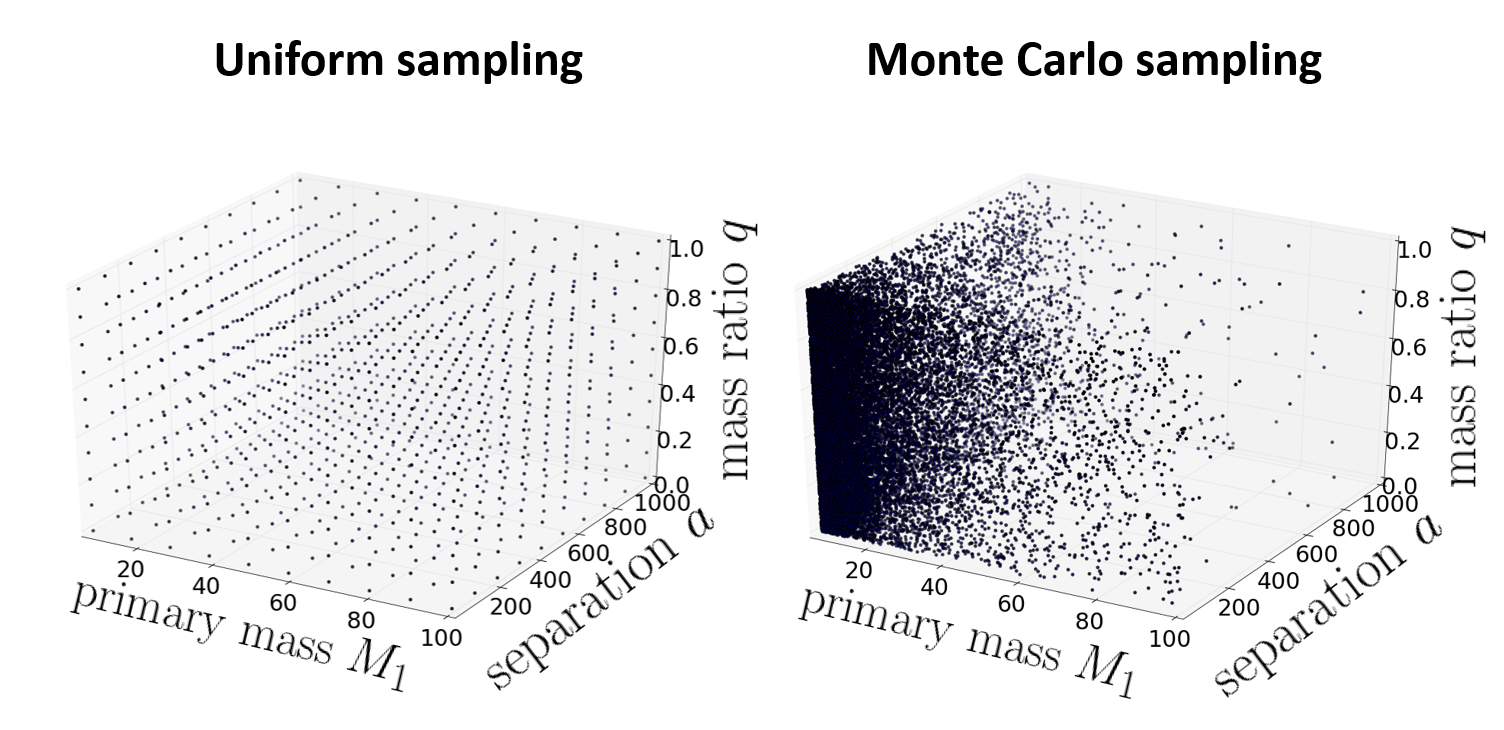
\includegraphics[width=\columnwidth]{sampling_methods.png}
    \caption{Example of   samples that are drawn (left)  uniformly distributed over the initial parameter space and (right) follow their birth distribution. The samples in the right plot are centred in the left corner since in the primary mass birth distribution used here low mass stars are much more common that high mass stars. }
    \label{fig:sampling_methods}
\end{figure}



\subsection{Adaptive importance sampling}
\label{subsec:aIS}
In the adaptive importance sampling (aIS) method, the  distribution from which the initial binaries are sampled is adaptively changed such that the computational time is spend more on the part of the initial parameter space that also contributes most to the information.
In other words, the adaptive importance sampling method reduces the sampling variance by sampling from a so-called \emph{instrumental distribution} that is more similar to the target distribution than the prior distribution,  this is shown in Fig.~(\ref{fig:intuitive}). Especially when simulating a process where a small part of the initial space produces the output of interest, changing the sampling distribution can significantly reduce the costs of the simulation. 

%.    The intuitive idea is thus to take an instrumental distribution that places  more sample points $\mathbf{x_i}$ in the part of the initial parameter space that contributes most to our output parameter space of interest (e.g. BBH mergers) 


\begin{figure}
	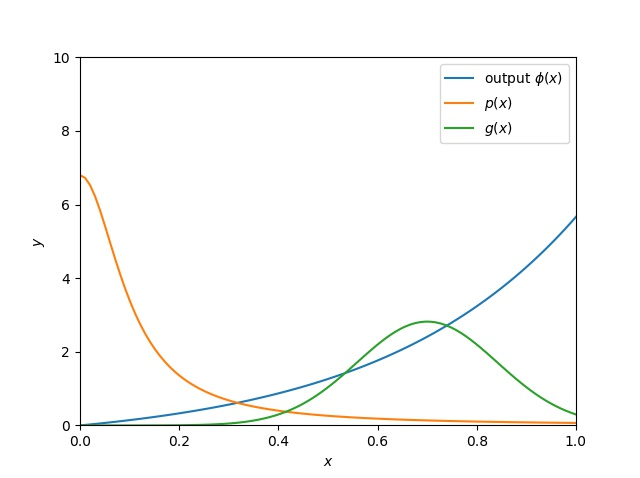
\includegraphics[width=\columnwidth]{intuitive.jpg}
    \caption{The intuitive idea of importance sampling is that often in the initial distribution function $p(x)$ only very few of the drawn samples will contribute to  the integral of the output function $phi(x)$ if $p(x)$ and $\phi(x)$ are dissimilar (especially in rare events). The idea of importance sampling is to sample instead from an instrumental distribution $g(x)$ such that a higher fraction of the drawn samples contribute to the estimate of the integral of $\phi(x)$. }
    \label{fig:example_figure}
    \label{fig:intuitive}
\end{figure}




The aIS method consists of three main steps which are shown in the scheme in Fig.~(\ref{fig:aIS_scheme}). 

\begin{itemize}
\item \textbf{Initial guess} \\
Since the initial parameters that will produce systems of a certain population are not known a priori, the initial parameter space has to be explored first. Therefore,  only for the first run, a first guess of where to draw the binary samples $\mathbf{x_f}$ in the initial parameter space has to be made. The most simplified choice would be to draw the first samples using the Monte Carlo sampling method.  



  

\item \textbf{Run simulation } \\ Then, initial  conditions for the binary systems are drawn from the initial guess distribution and the samples are run through the BPS model until a certain threshold number of binaries of a specific target population have been found. (e.g.  sample until 100 BBH mergers are found). 

\item \textbf{Improve sampling distribution} \\
Now that a first set of initial conditions $\{ \mathbf{x_i} \}_{i=1}^{N}$ is known to produce binary systems of the specific population of interest, i.e., $\phi(\mathbf{x_i}) = 1$ for all $i = 1, .., N$, we can improve the sampling distribution. 
This is done by defining the new sampling distribution $g(\mathbf{x_i})$ as the mixture of $N$ multivariate Gaussian distributions, where each Gaussian distribution $g_i$ is cantered around a successful outcome $x_i$. I.e.: 
%
\begin{equation}
    g(\mathbf{x}) = \sum _{i=1}^{K} \frac{1}{K} g_i(\mathbf{x}) = \frac{1}{K}  \sum _{i=1}^{K}  \mathcal{N}({\boldsymbol {\mu _{i},\Sigma _{i}}}), 
	\label{eq:instrumental-distribution}
\end{equation}
%
where each Gaussian distribution $\mathcal{N}({\boldsymbol {\mu _{i},\Sigma _{i}}})$ is equally weighted with $1/K$ in the mixture distribution. Since the Gaussians are distributed around the $\mathbf{x_f}$ that belonged to the target population, the means $\mu_i$ are given by $\mathbf{\mu_i} = \mathbf{x_i}$ for $i = 1, ..., K$. 

Furthermore, we scale the covariance matrix $\Sigma$  with the average expected distance between our initial sample points $ \mathbf{x_i}$ in the initial binary parameter space. This is chosen such that samples drawn from a Gaussian $\mathcal{N}({\boldsymbol {\mu _{i},\Sigma _{i}}})$  will generally fall in the space between the successful point  $x_i$ and its nearest neighbour.  For simplicity we choose $\Sigma_i = \Sigma$ for all $i$ and also adopt a diagonal covariance matrix for $\Sigma$ given by 
%
\begin{equation}
\Sigma = \begin{bmatrix} 
    \sigma_{1}^2 & 0 & \dots \\
    \vdots & \ddots & \\
    0 &        & \sigma_{d}^2 
    \end{bmatrix}, 
	\label{eq:covariance-matrix}
\end{equation}
%
where each $\sigma_k $  is given by
%
\begin{equation}
\sigma_k =  \frac{\|x_{k, \text{max}} - x_{k, \text{min}}\|}{(N_{\text{ini}})^{1/d}} \  \text{ for } k = 1,.. ,\text{d}.
	\label{eq:sigma-covariance-matrix}
\end{equation}
%
where $N_{\text{ini}}$ is the total number of initial samples used and $d$ is the dimension of the parameter space. 
\end{itemize}


\begin{figure}
	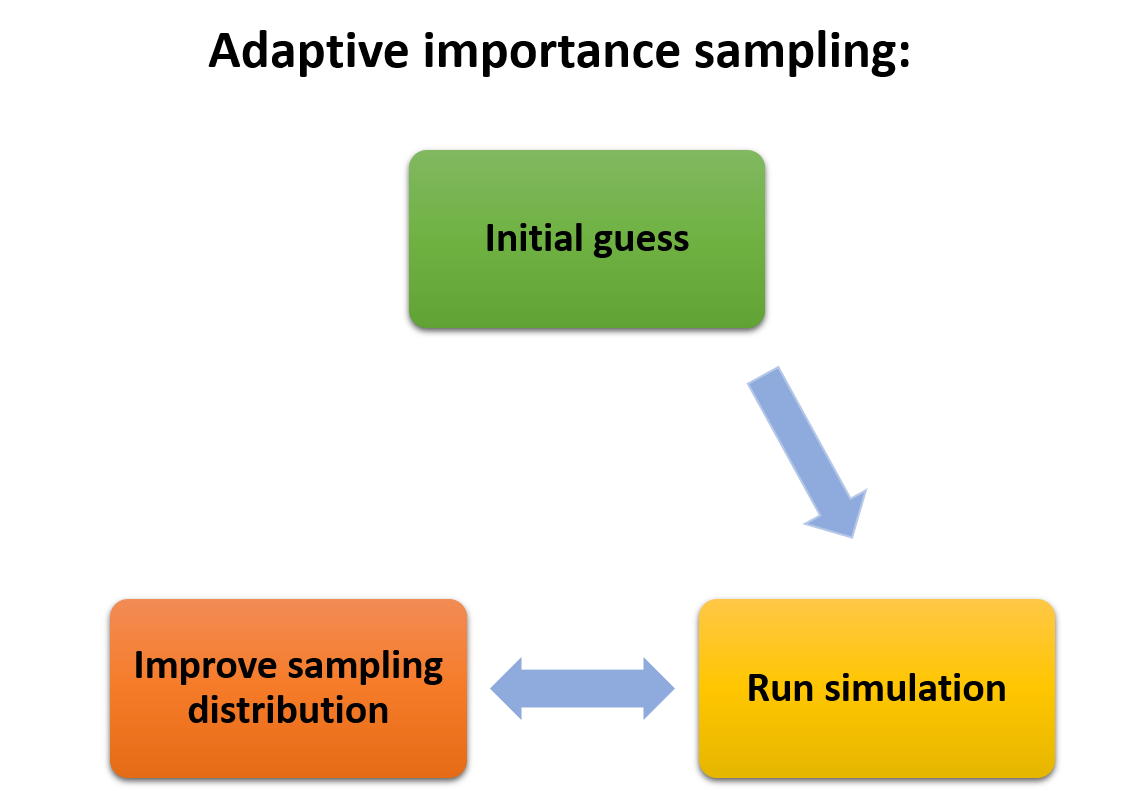
\includegraphics[width=\columnwidth]{aIS_scheme.png}
    \caption{ }
    \label{fig:aIS_scheme}
\end{figure}


To account for the change of the sampling distribution, weights are introduced that correct for the new distribution when calculating the distributions and moments of $\phi(\mathbf{x})$. The weights are given by 
%
\begin{equation}
w_k = p(\mathbf{x_i})/g(\mathbf{x_i}) .
\end{equation}
%
And thus, for example, the expectation value of  $\phi(\mathbf{x})$ using adaptive importance sampling is  given by
%
\begin{equation}
    \hat{I}[\phi(\mathbf{x})] = \frac{1}{K} \sum_{i=1}^{K} \phi(\mathbf{x_i}) \frac{p(\mathbf{x_i})}{g(\mathbf{x_i})}. 
	\label{eq:ISestimator}
\end{equation}





	



\subsection{Initial binary parameter space}
\label{subsec:BPS-prior}

Each binary system is characterized  in these simulations by the three initial parameters $\mathbf{x_i} = (M_{1,i},\ a_i, \ q_i). $ such that when assuming independent parameters the prior of   $\mathbf{x_i}$ is given by: 
%
\begin{equation}
p(\mathbf{x_i}) = p({M_{1,i}}) \ p({a_i}) \  p({q_i}).
\end{equation}
%
The distributions and parameter spaces of each of the three parameters is introduced below. 



The initial primary mass $M_{1,i}$ is given by a power law  
%
\begin{equation}
    p(M_1) = K_M M_1^{-\alpha},  \ M_{1,i} \in [M_{1,\text{min}} , M_{1,\text{max}} ]
	\label{eq:prior-IMF}
\end{equation} 
%
where $\alpha = 2.35$ is chosen to follow the Salpeter law and $K_M$ is the normalization constant. We choose the primary mass to be in the range $M_1 \in [7,100] M_{\odot}$ for astrophysical arguments.  \\

The separation $a_i$ is chosen to be uniform in log and 	its prior is given by
%
\begin{equation}
    p(a_i) = \frac{K_a }{a_i},   \ a_i \in [a_{\text{min}} , a_{\text{max}} ]
	\label{eq:prior-separation}
\end{equation} 
%
where we choose $[a_{\text{min}} , a_{\text{max}} ] =  [0.1,10^3]  $ AU and $K_a$ is the normalization constant. \\

The mass ratio $q$ is chosen to be flat and is given by

\begin{equation}
    p(q) =  \frac{1}{q_{\text{max}} - q_{\text{min}}} 
	\label{eq:prior-massratio}
\end{equation}



\subsection{More details about the code? }


%%\section{Methods old}
%Calculating informative properties of the outcome of  simulations such as the fraction of BBHs that produce GWs or their chirp mass distribution often involves calculating integrals. However, since in a simulation only a finite number of simulations are run, in practice it comes down to estimating the value of the integral from the evaluated simulations. The most used method to do this is the Monte Carlo method. The aim of this paper is to introduce a method that improves this estimation compared to the Monte Carlo method. Therefore, we will first introduce the Monte Carlo method before explaining the proposed method. 
%\subsection{Monte Carlo estimator}
%Let $\boldsymbol x = x_1,x_2,... x_d$  be a random variable of dimension $d$ and let $p(\boldsymbol {x})$ be the initial probability distribution function of $\boldsymbol {x}$.  Let $\phi(\boldsymbol{x}): \mathbb{R}^d \rightarrow \mathbb{R}$ be a function that evaluates the input variable $\boldsymbol {x}$ in the model $u(\textbf{x})$ and  maps it to an output of interest. For example, $u(\textbf{x})$ can represent the population synthesis model and  $\phi(\boldsymbol {x})$ can be the function that maps   the initial mass of a star to its final mass. 
%
%The basic principle of the Monte Carlo method is to generate a finite number of random samples $\mathbf{x}_1, \mathbf{x}_2,... \mathbf{x}_N$ that are identically and independently distributed from $p(\mathbf{x})$ and represent the distribution. The expectation value of $\phi(\mathbf{x})$ can then be estimated with the Monte Carlo method by 
%
%\begin{equation}
%    \hat{M}[\phi(\mathbf{x})] = \frac{1}{N} \sum_{k=1}^{N} \phi(\mathbf{x_k}) \approx \mathbb{E}[\phi(\mathbf{x})].
%	\label{eq:MCestimator}
%\end{equation}
%
%The Monte Carlo method estimator has a convergence rate of $O(\frac{1}{\sqrt{N}})$, which can be derived from the central limit theorem. Although the convergence rate is independent of the number of dimensions, it is also relatively slow: to decrease the error of  \eqref{eq:MCestimator} by a factor of ten, one needs to increase the number of samples by a factor of hundred. The goal of this paper is to try to improve the estimator  \eqref{eq:MCestimator} focusing on simulating rare events with binary population synthesis models.
%
%
%
%
%
%\subsection{Importance sampling}
%
%Importance sampling can reduce the error of estimation obtained after a given number of evaluations (and therefore the costs of the simulation), by taking the random variables $\mathbf{x}_1, \mathbf{x}_2,... \mathbf{x}_N$ from a so-called \emph{instrumental distribution} $g(\mathbf{x})$, which is a different distribution than the prior distribution $p(\mathbf{x})$ but acts on the same parameter space. The idea is to take an instrumental distribution that samples more sample points $\mathbf{x_k}$ in the part of the initial parameter space that contributes most to our output parameter space of interest (e.g. BBH mergers). Especially when simulating a process where a small part of the initial space produces the output of interest (i.e. a rare event), changing the sampling distribution can significantly reduce the costs of the simulation. The intuitive idea of importance sampling is shown in Fig.~(\ref{fig:intuitive}).
%
%However, since the sampling distribution is changed, weights are introduced that correct for this in the estimation of the expectation of $\phi(\mathbf{x})$. If $\mathbf{x}$ is initially distributed by $p(\mathbf{x})$ and   the instrumental distribution $g(\mathbf{x})$ is used, the estimator for the expectation value of  $\phi(x)$ via importance sampling is  given by 
%
%\begin{equation}
%    \hat{I}[\phi(x)] = \frac{1}{N} \sum_{k=1}^{N} \phi(x_k) \frac{p(x_k)}{g(x_k)},
%	\label{eq:ISestimator}
%\end{equation}
%
%
%where $p(\mathbf{x_k})/g(\mathbf{x_k}) = w_k$ are the weights.
% 
%
%\begin{figure}
%	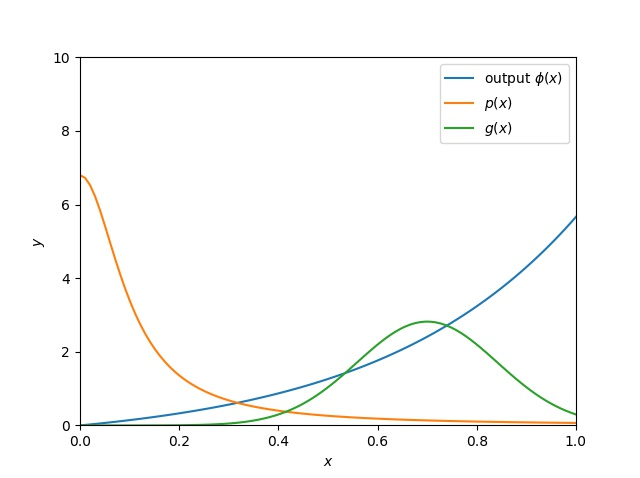
\includegraphics[width=\columnwidth]{intuitive.jpg}
%    \caption{The intuitive idea of importance sampling is that often in the initial distribution function $p(x)$ only very few of the drawn samples will contribute to  the integral of the output function $phi(x)$ if $p(x)$ and $\phi(x)$ are dissimilar (especially in rare events). The idea of importance sampling is to sample instead from an instrumental distribution $g(x)$ such that a higher fraction of the drawn samples contribute to the estimate of the integral of $\phi(x)$. }
%    \label{fig:example_figure}
%    \label{fig:intuitive}
%\end{figure}
%
%
%
%\subsection{Adaptive importance sampling}
%\label{sec:IS}
%Often the output function $\phi(\mathbf{x})$ is not known before running any simulations, hence the instrumental distribution $g(\mathbf{x})$ cannot be determined on beforehand. Instead, we use an adaptive sampling scheme that adaptively samples from an instrumental distribution $g_i(\mathbf{x})$ that is based on earlier model outcomes. The basic algorithm of the method works as follows:
%
%\begin{enumerate}
%\item Sample random variables $\mathbf{x}_1, \mathbf{x}_2,... \mathbf{x}_N$ from the initial distribution $p(\mathbf{x})$ and evaluate $\phi(\mathbf{x_k})$ for all $k = 1,2,.. N_\text{ini}$ until a certain threshold is reached.  This threshold can for instance be a number of successful evaluations e.g. ``\emph{when $100$ binary black hole mergers are simulated}'' or  ``\emph{when $100$ binary black holes with chirp mass above $20$ $M_{\odot}$ are simulated}''.  In each case there is an initial number $N_{\text{ini}}$ of sample points in parameter space needed to produce $N_s$ initial successes of the model (where $N_s = 100$ in our examples). 
% 
%\item   Now define the instrumental distribution $g_1(\mathbf{x})$ as a mixture of $N_\text{s}$ Gaussian distributions around the $N_\text{s}$ successful sample points in the initial parameter space. %This idea is schematically shown in Figure~(\ref{fig:Gaussians}).
%
%The instrumental distribution is then described by 
%\begin{equation}
%    g_{1}(\mathbf{x}) = \sum _{i=1}^{N_{\text{s}}} \frac{1}{N_{\text{s}}} \mathcal{N}({\boldsymbol {\mu _{i},\Sigma _{i}}}), 
%	\label{eq:instrumental-distribution}
%\end{equation}
%where each Gaussian distribution $\mathcal{N}({\boldsymbol {\mu _{i},\Sigma _{i}}})$ is equally weighted with $1/N_{\text{s}}$ in the mixture distribution. The idea is thus that each Gaussian distribution $\mathcal{N}({\boldsymbol {\mu _{i},\Sigma _{i}}})$ as part of the mixture $g(\textbf{x})$ is drawn around one ``successful'' sample point $\mathbf{x_i}  \in \{ \mathbf{x_i}\}_{i=1}^{i = N_{\text{s}}}$. This implies that the means $\mathbf{\mu_i}$ of the individual Gaussians in Equation~(\ref{eq:instrumental-distribution}) are given by
%
%\begin{equation}
%    \mathbf{\mu_i} = \mathbf{x_i} \hspace{0.5cm} \text{for } i = 1,2,... , N_{\text{s}}.
%	\label{eq:IS-mu}
%\end{equation}
%explores mostly the parameter space
%The covariance matrix $\Sigma$ is chosen to scale with the average expected distance between two sample points $\{ \mathbf{x_k} \}_{k=1}^{k=N_{\text{ini}}}$ in our initial parameter space. This is chosen such that samples drawn from a Gaussian $\mathcal{N}({\boldsymbol {\mu _{i},\Sigma _{i}}})$  will generally fall in between the successful point (and mean of the Gaussian) $x_i$ and its nearest neighbour.  For simplicity we choose $\Sigma_i = \Sigma$ for all $i$ and also a diagonal covariance matrix for $\Sigma$ given by 
%
%\begin{equation}
%\Sigma = \begin{bmatrix} 
%    \sigma_{1}^2 & 0 & \dots \\
%    \vdots & \ddots & \\
%    0 &        & \sigma_{d}^2 
%    \end{bmatrix}, 
%	\label{eq:covariance-matrix}
%\end{equation}
%
%where each $\sigma_k $  is given by
%\begin{equation}
%\sigma_k =  \frac{\|\text{max}_k - \text{min}_k \|}{(N_{\text{ini}})^{1/d}} \  \text{ for } k = 1,.. ,\text{d}.
%	\label{eq:sigma-covariance-matrix}
%\end{equation}
%
%In Equation~(\ref{eq:sigma-covariance-matrix}) $ \text{max}_i $ and $ \text{min}_i $ are the maximum and minimum range of $x_i$. (NB: for later generations of $g(\mathbf{x})$ $N_{\text{ini}}$ is changed into $N_{\text{tot}}$, the total number of samples that were drawn and evaluated in the simulation at this stage). 

%
%\item New samples $\mathbf{x_1}, \mathbf{x_2},... \mathbf{x_K}$ are drawn from the instrumental distribution $g_1(\mathbf{x})$ given by Equation~(\ref{eq:instrumental-distribution}) and evaluated in the function $\phi(\mathbf{x})$. Since we are now drawing samples from the instrumental distribution that is focused in the initial parameter space around the initial samples that produced an outcome of interest, the samples that we draw from the instrumental distribution will more often also produce the rare event - as long as the output space does not behave too chaotic or stochastic. 
%
%%\item \textbf{(TO CHANGE)}: I should add that we reject samples when they are drawn outside of parameter space, and the fact that we don't have to normalize our distribution for this at all as in the importance sampling estimator the normalizations of the instrumental distribution cancels out. 
%
%\item From these evaluations the expected value of $\phi(\mathbf{x})$ can be estimated using Equation~(\ref{eq:ISestimator}) and the uncertainty of the estimation. %And the uncertainty is estimated by Equation() \textbf{TO DO}: [Add equations for uncertainties]. 
%
%\item Increase the number of sample points, or repeat steps (ii) to (iv) to update the instrumental distribution (which will converge to the distribution of the rare event) until a certain error is reached. 
%\end{enumerate}
%



%\begin{figure}
%	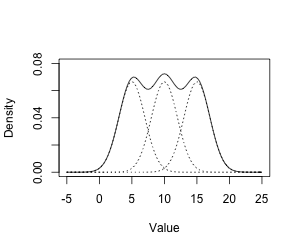
\includegraphics[width=\columnwidth]{Gaussians.png}
 %   \caption{NEED TO CHANGE THIS FIG. Here we will show the intuitive idea of why we sample from a mixture of Gaussians around our hits of BBH mergers)}
  %  \label{fig:Gaussians}
%\end{figure}




\section{A test case application: BBH mergers}
%
Consider for $u(\mathbf{x})$ the binary population synthesis model COMPAS  that simulates the evolution of binary systems and focuses on the evolution to compact objects such as neutron stars and black holes. 
Suppose the initial parameter space is 3-dimensional (d$=3$) with parameters $\mathbf{x} = (M_1, a, q)$, where $M_1$ is the initial mass in solar mass $M_{\odot}$ of the most massive star (the primary) in the binary system, $a$ is the initial separation of the binary given in AU and $q$ the initial mass ratio of the binary, i.e. $q = M_2/M_1$ where $M_2$ is the mass of the secondary.  
%
%
Suppose the outcome of interest is the fraction of binary black hole mergers $f_{\text{BBH merger}}$, our output function $\phi(M_1,a,q)$ can then be given by 
%
\begin{equation}
    \phi({M_1,a,q}) = \begin{cases} 
    1  \ \text{if } u(M_1,a,q) \text{ produces a BBH merger} \\
    0  \ \text{else}     \end{cases}
	\label{eq:ex-output-phi}
\end{equation} 
%
The fraction of the initial parameter space that will produce BBH mergers when evaluated in the model (i.e. $f_{\text{BBH merger}}$) can then be estimated by using Equation~(\ref{eq:ISestimator}) by simulating N binary systems with the adaptive importance sampling method. In other words 
%
\begin{equation}
    f \approx \hat{I}[\phi(M_1,a,q)] = \frac{1}{N} \sum_{i=1}^{N} \phi(M_1,a,q) \frac{p(M_1,a,q)}{g(M_1,a,q)}. 
	\label{eq:ex-ISestimator}
\end{equation}

Assuming  $p({M_1,a,q}) = p(M_1) \  p(a)  \  p(q)$ the prior is given by the product of the individual probability distribution functions which are summarized in Table  \ref{my-label}. Using these distributions, we find
%
%\begin{itemize}

%\item The primary mass $M_1$ (Kroupa):
%\begin{equation}
%    p(M_1) \propto M_1^{-\alpha} 
%	\label{eq:prior-IMF}
%\end{equation} 
%where $\alpha = 2.35$. We choose the primary mass to be in the range $M_1 \in [7,100] M_{\odot}$ for astrophysical arguments. (REFs) \\
%
%\item The separation $a$ 
%\begin{equation}
%    p(a) \propto 1/a  
%	\label{eq:prior-separation}
%\end{equation} 
%where $a \in [0.1,10^3]  $ AU (REFs) \\
%
%\item the mass ratio $q$ 
%\begin{equation}
%    p(q) \propto 1 
%	\label{eq:prior-separation}
%\end{equation}
%(REFs) 
%\end{itemize}
\begin{equation}
  p(M_1,a,q) \propto \frac{M_1^{-2.35}}{a} 
	\label{eq:ex-full-prior}
\end{equation}
%

\begin{table}[]
\centering
\caption{Summary of properties initial parameters}
\label{my-label}
\begin{tabular}{|l|l|l|}

parameter & pdf & range \\ \hline
$M_1$     &  $p(M_1) \propto M_1^{-2.35}$    & $[7,100] \text{M}_{\odot} $      \\ \hline
$a$       &  $ p(a) \propto 1/a$             & $[0.1,10^3] $AU            \\ \hline
$q$       &   $1$                   		   &  $[0,1] $                  \\ \hline
\end{tabular}
\end{table}
%  
%  
Following the algorithm described in Section~(\ref{sec:IS}) we define the instrumental distribution
\begin{equation}
    g_{1}({M_1,a,q}) = \sum _{i=1}^{N_{\text{s}}} \frac{1}{N_{\text{s}}} \mathcal{N}({\boldsymbol {\mu _{i},\Sigma}}).
	\label{eq:exampple-g(x)}
\end{equation}

By filling in Equations (\ref{eq:ex-output-phi}), (\ref{eq:ex-full-prior}) and (\ref{eq:exampple-g(x)}) into Equation~(\ref{eq:ex-ISestimator}) we have all the ingredients for the importance sampling estimator. 




%%%%%%%%%%%%%%%%%%%%%%%%%
%%%%%%%%%%%%%%%%%%%%%%%%
\section{Preliminary results}
To test how well the adaptive importance sampling method works we run a large Monte Carlo simulation with more than $10^7 $ sample points to estimate the fraction of the BBH mergers within the mentioned initial parameter space up to error $1.4 \cdot 10^{-5}$. We find $f = 0.002797 \pm 14$. We then run the simulation using the adaptive importance sampling method with different number of total samples $N_{\text{tot}}$ and estimate the fraction of BBH mergers with Equation (\ref{eq:ex-ISestimator}) and compare this with the value for the fraction found by the large Monte Carlo run. We also run the simulation with $N_{\text{tot}}$ samples using the crude Monte Carlo method as given in Equation~(\ref{eq:MCestimator}) and add the estimated  error from the true fraction to the plot. 

At the moment of writing, the full code that works for the binary population synthesis model COMPAS is still in progress. Nevertheless, we have tested the adaptive importance sampling on a test problem and show in this section the results of these tests. 

For the preliminary tests, we created a 3-dimensional parameter space $\Omega_3 = [-1,1]^3$. We defined $\phi(x)$ to be a function on $\Omega_3$ such that it maps a fraction $f \sim 0.00345 $ of the full parameter space  to 1 whilst the rest maps to zero (i.e. $\phi(x) = 1$ on three spheres in $\Omega_3$ and $0$ else). This value for the fraction is chosen such that it is representative for the fraction of BBHs that merges within Hubble time in simulations run with population synthesis model COMPAS. The regions that map to zero are defined as three spheres within the parameter space, which are shown in Figure \ref{fig:spheres}.


We initially draw samples from a 3D uniform distribution and after thirty of the initial samples fall in the volume of the spheres (and thus evaluate to $1$ instead of $0$) the initial sampling is stopped and we change to the adaptive importance sampling scheme. 
To test the performance of the method, we run the simulation several times for multiple $N_{\text{tot}}$ and compute the error. We compare the results with the Monte Carlo method and the true value of the fraction, which in this case can be determined analytically by the volume of the spheres. The results are shown in Figure \ref{fig:example_figure}.
%
%
\begin{figure}
	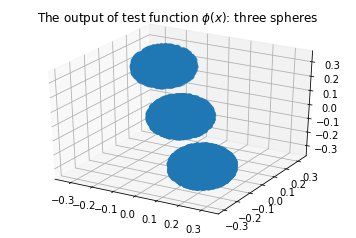
\includegraphics[width=\columnwidth]{spheres}
    \caption{	Plot of the test function $\phi(x)$ that is used to obtain the preliminary results. $\phi(x)$ maps all $x$ within the sphere (blue dots) to $1$ and the rest to zero. The volume of the spheres is chosen such that the fraction of successful samples (blue dots) is representative for COMPAS.}
    \label{fig:spheres}
\end{figure}
%
%
%  
From this Figure  it can be seen that: 
\begin{itemize}
\item The error of the estimation for both methods is smaller for larger $N_{\text{tot}}$. This is expected as more simulation runs, and thus more computational cost, will usually give better results. 
\item The errors of the adaptive importance sampling method are always smaller than the errors from the Monte Carlo method. This means that with the same number of runs, the adaptive importance sampling method gives better results than the Monte Carlo method. 
\item The adaptive importance sampling method is a factor Y more efficient: the same error is obtained with Y times less sample points. 
\end{itemize} 

\begin{figure}
	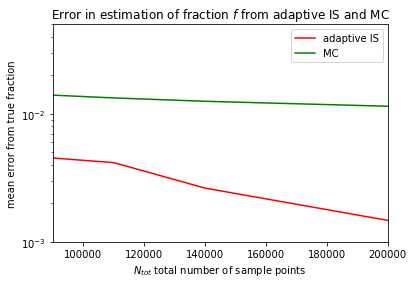
\includegraphics[width=\columnwidth]{figure22}
    \caption{Mean absolute error of the adaptive importance method (red) and the Monte Carlo method (green) as a function of the number of simulations run $N_{\text{tot}}$ (i.e. the computational costs). These results are still preliminary as it obtained from tests with the toy population synthesis model. We are working on performing a similar test when the code is fully adapted for binary population synthesis codes like COMPAS. }
    \label{fig:example_figure}
\end{figure}


%\section{Conclusions}



\section*{Acknowledgements}

We thank the the Kavli Foundation, Niels Bohr institute and DARK Cosmology Centre in Copenhagen for their hospitality and for organising the Kavli summer school in gravitational waves astrophysics 2017. This work could not have been done without their support. 

%%%%%%%%%%%%%%%%%%%%%%%%%%%%%%%%%%%%%%%%%%%%%%%%%%

%%%%%%%%%%%%%%%%%%%% REFERENCES %%%%%%%%%%%%%%%%%%

% The best way to enter references is to use BibTeX:

\bibliographystyle{mnras}
\bibliography{my_bib} % if your bibtex file is called example.bib


% Alternatively you could enter them by hand, like this:
% This method is tedious and prone to error if you have lots of references
%\begin{thebibliography}{99}
%\bibitem[\protect\citeauthoryear{Author}{2012}]{Author2012}
%Author A.~N., 2013, Journal of Improbable Astronomy, 1, 1
%\bibitem[\protect\citeauthoryear{Others}{2013}]{Others2013}
%Others S., 2012, Journal of Interesting Stuff, 17, 198
%\end{thebibliography}

%%%%%%%%%%%%%%%%%%%%%%%%%%%%%%%%%%%%%%%%%%%%%%%%%%

%%%%%%%%%%%%%%%%% APPENDICES %%%%%%%%%%%%%%%%%%%%%

%\appendix

%\section{Some extra material}


%%%%%%%%%%%%%%%%%%%%%%%%%%%%%%%%%%%%%%%%%%%%%%%%%%


% Don't change these lines
\bsp	% typesetting comment
\label{lastpage}
\end{document}

% End of mnras_template.tex
